\chapter{Hybrid evolutionary approach}
\label{chap:methodology}
%\minitoc

An evolutionary algorithm is a technique bio-inspired by the evolution of the espicies. It was proposed by John Holland early in the 70's (Holland, 1975). This algorithm seeks to evolve a population of individuals that represent solutions to the problem through genetic operators such as crossover, mutations and selection. The population generated in each iteration is evaluated and then the individuals with a better fitness are chosen for the next generation with more chance.

\section{Hybrid genetic algorithm}

A hybrid evolutionary algorithms or hybrid genetic algorithms are a very popular techniques that offers practical advantages to deal with complex and hardly optimization problems. Grosan (Grosan, 2007) present a review of hybrid genetic architectures frecuently used. 

Hybridization can be performed using prior knowledge, heuristics, local search, other techniques. We use it to carry out local search through rollout algorithm. Some times, a hybrid genetic algorithm which combine other technique to local search is known as memetic algorithm.

Generally, the purpose of hibridization is:

\begin{itemize}
 \item Improve the performance of the evolutionary algorithms.
 \item Improve quality of solutions obtained by evolutionary algorithm
 \item Incorporate evolutionary algorithm as part of a large system
\end{itemize}

Evolutionary algorithm behavior is determined by the exploitation and exploration; In exploitation local search is performed to improve solutions, and exploration avoid local optimum extending the search space, our implementation of memetic algorithm works to keep these relation throughout the run. So, in this application hybridazation not only improve the quality of the solutions obtained by evolutionary algorithm, also is assembly as an framework for rollout algorithm in order to avoid local optimum.


\subsection{A basic genetic algorithm for vehicle routing problem with stochastic demands}

We show an example of basic GA in general form in figure \ref{fig:ga_basic}. First, an initial population is selected and fitness function is assessed for each individual in the population. In order to produce a new population for the next generation, crossover and mutation operators are applied to individuals allowing those who have better fitness function to get more chances to reproduce themselves. In the selection stage, offspring's fitness is evaluated to choose the individuals to integrate the new population; individuals with competitive fitness regarding to the population have more probability to be selected. These steps are repeated until stopping criteriums are resolve.

\begin{figure}[!htbp]
  \begin{center}
   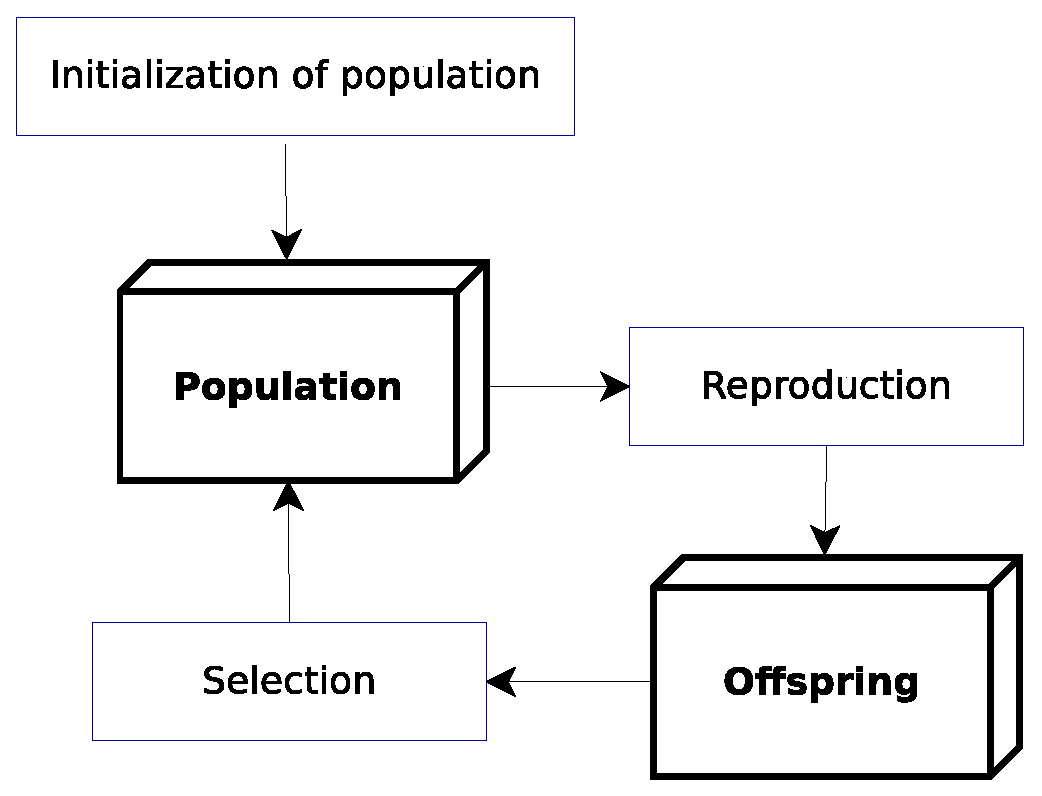
\includegraphics[width=0.6\textwidth]{Images/Chapter3/ga_basic.eps}
  \end{center}
    \caption{Basic genetic algorithm}\label{fig:ga_basic}
\end{figure}

\subsubsection*{Initialization}

We represent an individual in the population as a policy tour $\pi^\mathcal{C}$ whose fitness is the expected distance $\tilde{J}_{\pi^\mathcal{C}}$ computed using the algorithm $\Gamma$ \ref{algo:expecteddistance}.

The initial population $P_0$ with an fixed size $|P_0| = n$, is obtained using the cyclic heuristic in $O(n)$ time. It performs in order to reduce the computational cost since we can evaluate fitness to $P_0$ in $O(n)$ time when rollout is accomplished under some individual in the population.


\subsubsection*{Crossover}

The crossover operator $\circledast$ consist in to select two different individuals $I^{P_k}_i$ and $I^{P_k}_j$ with probability dependently of their fitness value respectively; meanwhile, a random cut point $\rho \in [1,n]$ is selected uniformly. So, a new individual raise to concatenate the subsequence $I^{P_k}_i[1..\rho]$ with the subsequence $I^{P_k}_j[\rho+1,..,n]$. 

A crossover operation can yield an new individual that represents an unfeasible policy. However, we implement this operator to run in time $O(n^2)$ and guaraneeing only feasible solutions as a result.


\subsubsection*{Mutation}

This operator performs three types of mutation with same probability to produce and individual in the offspring: swap two elements of policy selected randomly, flip a random subsequence of policy or shift the policy an random number of times.

The mutation of an individual can happened with probability $Prob_m = 0.04$ in the experiments presented in this document and it compute in $O(1)$ time.


\subsubsection*{Selection of the new population}

New population originates as a result of crossover and mutation operators. However, the evolutionary algorithm also obtain individuals to the offspring performing the cyclic heuristic. Hence, those who have better fitness can be choosen with more chance to integrate the new population.

In order to punish generation which dicrease the fitness and reward to those who increase this value respect to the previos generation the size or number of individuals available to the next generation changes.

Let $\Delta^{P_k}_{E'}$ be the rate of fitness change in the generation $P_k$, i.e.

\begin{equation}\label{eq:improve_fitness}
 \Delta^{P_k}_{E'} = \frac{\bar{\Gamma}_{P_{k-1}} - \bar{\Gamma}_{P_k}}{\bar{\Gamma}_{P_{k-1}}} 
\end{equation}

where $\bar{\Gamma}_{P_k}$ is the best expected distance obtained by an individual in the generation $k$.

Then, the size of the next population $P_{k+1}$ is computed so:

\begin{equation}\label{eq:population_size}
 ||P_{k+1}|| = \left \{ \begin{array}{ll}
  \lfloor  \min\{n(1+\alpha), ||P_{k}||(1+\alpha)\} \rfloor, & \text{if } \Delta^{P_k}_{E'} > 0\\
  \lceil \max\{n\alpha, ||P_{k}||\alpha\} \rceil, & \text{if } \Delta^{P_k}_{E'} < 0
  ||P_{k}||, \text{in other case.}
  \end{array} \right.
\end{equation}


where $\alpha$ is a tuneable parameter which should be fixed in the range $(0,1]$ depending of computational resources. Consequently it reward a offspring that improve the quality of the solutions in comparison to theirs parents, increasing the population size at most an $\alpha$ times the size. Otherwise, when the quality of the solutions decrease respect to the previos generation, the size of population is punished decreasing it at least an $\alpha$ factor of the size of population. The figure \ref{fig:ga_basic_i_30r1} shows results of basic genetic algorithm applied to one instance with $\alpha = 0.5$, the last chart below on the right side of figure exhibit the size of population for each generation.

\begin{figure}[!htbp]
  \begin{center}
   \includegraphics[width=0.9\textwidth]{Images/Chapter3/i_30r1_regular.eps}
  \end{center}
    \caption{Basic genetic algorithm applied to instance of 30 customers. The second image in the first row ilustrate the last population and the next image shows the best solution finded. }\label{fig:ga_basic_i_30r1}
\end{figure}

\subsubsection*{Stopping criterion}

Finally, the evolutionary algorithm runs until reach a fixed number or iterations $\kappa$. Nevertheless, it can stop once accopmlish $\mathbf{m}$ number of consecutive iterations whitous a significative change, i.e., $|\Delta^{P_k}_{E'}|\leq \varepsilon$

% \subsubsection{Crossover - EAX}

% Edge assembly crossover

% \subsubsection*{Mutation}

% Swap

\subsubsection*{local search}


A classic genetic algorithm does not yield competitive results itself, due to simple GA does not exploit problem knowing to produce high quality solutions. To be effective, we combine local search methods.


Often hybridazation is included in inicialization and reproduction operators.

local search can be incorporated in the initial population or among the offspring.

\subsubsection*{Performance of the genetic algorithms}

This section describes the algorithm performance for a specific problem instance with 10 customers and a factor $f'=1$, the customers' location and demand value (known when the vehicle arrive to the customer location) are showed in the figure \ref{fig:customer_n10_f1_s1}.


%\begin{figure}[!htbp]
%  \begin{center}
%    \includegraphics[width=0.9\textwidth]{Chapitre3/n10_f1_s1_customers}
%  \end{center}
%    \caption{Instance features: $n = 10$, $seed = 1$, $f' = 1$}\label{fig:customer_n10_f1_s1}
%\end{figure}

The genetic algorithm outcome for the instance problem described above is presented in the figure \ref{fig:tour_n10_f1_s1}, the red line describes the route, the segmented black line represents returns to the depot for replenishment, this tour was selected as the best solution found in 100 iterations of the GA.

%\begin{figure}[!htbp]
%  \begin{center}
%    \includegraphics[width=0.9\textwidth]{Chapitre3/n10_f1_s1_tour}
%  \end{center}
%      \caption{e.g best tour found by the GA: $n = 10$, $seed = 1$, $f' = 1$}\label{fig:tour_n10_f1_s1}
%\end{figure}

The figure \ref{fig:improve_n10_f1_s1} shows the improving of the objective function found, the chart shows the lesser total cost history, when a better value is found the line fall, therefore we can see the improving is given among the iteration 25 and 40, after this iterations the algorithm converges and it's not found a better solution.

%\begin{figure}[!htbp]
%  \begin{center}
%    \includegraphics[width=0.9\textwidth]{Chapitre3/n10_f1_s1_history}
%  \end{center}
%      \caption{e.g improvement solution: $n = 10$, $seed = 1$, $f' = 1$}\label{fig:improve_n10_f1_s1}
%\end{figure}

%\section{Memetic Algorithm}

%GA that use local search

%\section{Non-dominated Genetic Algorithm}

